

\section{Results}  \label{sec:ExperimentalResults}



\subsection{DeepReDuce Pareto Analysis}
Figure~\ref{fig:ParetoFrontier} shows that 
DeepReDuce advances the ReLU count-accuracy Pareto frontier.
In this section, we present a detailed analysis and
quantify the benefit of networks along the frontier.
Table~\ref{tab:ParetoPoints} shows the details of the 
DeepReDuce Pareto points in Figure~\ref{fig:ParetoFrontier}.
Pareto points are shown in order of highest to lowest accuracy.
The primary takeaway from the table is that each of our optimizations (Culling, Thinning and Reshaping) are represented on the Pareto front, indicating that each is critical to obtaining the best results. 
Second, as mentioned in Section~\ref{sec:Reshaping}, Reshaping optimizations are most helpful at lower ReLU budgets, while Culling and Thinning dominate higher ReLU budget points.
This observation reaffirms that the order we apply our optimizations performs well.

We focus on CIFAR-100 first to best compare against prior work. Table~\ref{tab:R18OnTinyImageNet} provides the same data using the TinyImageNet dataset for ResNet18 and the criticality evaluation results are shown in Table \ref{tab:ResNetBlockDropout}. The data validates the effectiveness and hints at the general applicability of DeepReDuce.
Similar to the CIFAR-100 results, we found ReLUs in the initial layer 
(e.g., $S_1$) to be least critical while ReLUs in the intermediate layers (specifically ReLUs in penultimate stage) are most critical.


{\bf Accuracy per ReLU:}
Given that ReLU minimization and accuracy are competing objectives,
it is interesting to understand network design tradeoffs as accuracy per ReLU.
In the final column of Table~\ref{tab:ParetoPoints} and Table \ref{tab:R18OnTinyImageNet} 
we report each networks' accuracy per kilo-ReLU on CIFAR-100 and TinyImageNet datasets.
When ranking networks with respect to ReLU count (highest to lowest),
we observe accuracy per ReLU increases as ReLU count decreases.
In the extreme, the worst performing  CIFAR-100 network (Table~\ref{tab:ParetoPoints}) is 13.9\% less accurate than the most accurate network but also uses 32$\times$ fewer ReLUs, resulting in 26.2$\times$ more accuracy per kilo-ReLU. 
Similarly, the lowest accurate network on TinyImageNet (Table \ref{tab:R18OnTinyImageNet}) is 22.7\% less accurate but 74.7$\times$ fewer ReLU count than the most accurate network, resulting in 48.8$\times$ more accuracy per kilo-ReLU.

We believe this is a beneficial property for ReLU optimizations like DeepReDuce.
It implies that as fewer ReLUs are used, each contributes more to accuracy,
picking up the slack.
Moreover, while it takes many ReLUs to train a highly-accurate network,
accuracy degrades slowly as significant quantities of ReLUs are dropped.
%The gracefulness in decline is likely in part due to DeepReDuce's careful selection of
%which ReLUs to elide.
This suggests that a natural robustness to ReLU dropping may be a property of neural networks
that designers can leverage to optimize networks for private inference.


\begin{table} [t] \centering
\caption{Comparison of DeepReDuce and the state-of-the-art
in private inference: CryptoNAS \cite{ghodsi2020cryptonas} and DELPHI \cite{mishra2020delphi}.
Results show that DeepReDuce strictly outperforms both solutions at various ReLU counts.
Acc. is top-1 accuracy on CIFAR-100 and Lat. is inference time in seconds.}
\label{tab:SOTAcomparison} 
\resizebox{0.48\textwidth}{!}{
\begin{tabular}{cccccccccc} \toprule
\multirow{2}{*}{ } & \multicolumn{3}{c}{ SOTA } & \multicolumn{3}{c}{ DeepReDuce } & \multicolumn{3}{c}{ Improvement } \\
\cmidrule(lr{0.5em}){2-4}  
\cmidrule(lr{0.5em}){5-7} 
\cmidrule(lr{0.5em}){8-10} 
& ReLUs & Acc.(\%) & Lat.(s) & ReLUs & Acc.(\%) & Lat.(s) & ReLU  & Acc.(\%) & Lat.(s) \\ \toprule
\multirow{4}{*}{  \rotatebox[origin=c]{90}{CryptoNAS} } & 344K & 75.5 & 7.50 & 197K & 75.50 & 3.94 & 1.75$\times$ & 0.0 & 1.9$\times$ \\
& 100K & 68.7 & 2.30 & 28.6K & 68.70 & 0.738 & {\bf 3.5$\times$} & 0.0 & 3.1$\times$ \\
& 86K & 68.1 & 2.00 & 28.6K& 68.70 & 0.738 & 3$\times$ & 0.6 & 2.7$\times$ \\
& 50K & 63.6 & 1.67 & {\bf 12.3K} & {\bf 65.00} & {\bf 0.455} & 4$\times$ & 1.4 & 3.7$\times$ \\ \midrule
\multirow{3}{*}{ \rotatebox[origin=c]{90}{DELPHI} } & 300K & 68 & 6.5 & 28.7K & 68.70 & 0.738 & 10.5$\times$ & 0.7 & 8.8$\times$ \\
& 180K & 67 & 4.44 & 24.6K & 68.41 & 0.579 & 7.3$\times$ & 1.4 & 7.7$\times$ \\
& 50K & 66 & 1.23 & {\bf 49.2K} & {\bf 69.50} & {\bf 1.19} & 1$\times$ & {\bf 3.5} & 1$\times$ \\
\bottomrule
\end{tabular}}
\vspace{-2em}
\end{table}


%\begin{tabular}{c|cc|cc|cc} \toprule
%\multirow{2}{*}{ } & \multirow{2}{*}{ \#ReLUs } & \multirow{2}{*}{ Acc(\%) } & \multicolumn{2}{c|}{ DeepReDuce } & \multicolumn{2}{c}{ Improvement } \\
%& & & \#ReLUs & Acc (\%) & ReLU ($\downarrow$) & Acc(\%$\uparrow$) \\ \toprule
%\multirow{4}{*}{ CryptoNAS } & 344K & 75.5 & 196.61K & 75.50 & 1.75$\times$ & - \\
%& 100K & 68.7 & 28.67K & 68.70 & 3.5$\times$ & - \\
%& 86K & 68.1 & 28.67K & 68.70 & 3$\times$ & 0.60 \\
%& 50K & 63.6 & {\bf 12.29K} & {\bf 65.00} & {\bf 4$\times$} & 1.40 \\ \midrule
%\multirow{3}{*}{ DELPHI } & 300K & 68 & 28.67K & 68.70 & 10.5$\times$ & 0.70 \\
%& 180K & 67 & 24.58K & 68.41 & 7.3$\times$ & 1.41 \\
%& 50K & 66 & {\bf 49.15K} & {\bf 71.10} & 1$\times$ & {\bf 5.10} \\ 
\begin{figure}[t] \centering
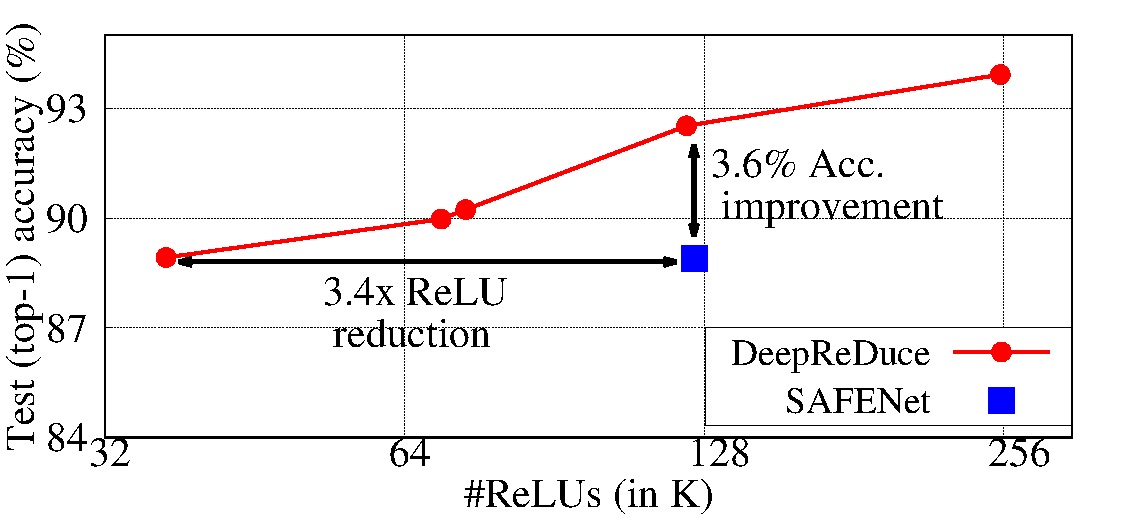
\includegraphics[scale=0.45]{Figures/ParetoFrontier_vgg16}
\vspace{-2em}
\caption{
Performance comparison of VGG16 DeepReDuce model and SAFENet on CIFAR-10. The DeepReDuce-optimized VGG16 models outperform SAFENet-optimized VGG16 by a huge margin at both iso-accuracy and iso-ReLU.}
\vspace{-2em}
\label{fig:ParetoFrontierVGG16}
\end{figure}



\subsection{DeepReDuce Outperforms Prior Work}
Table~\ref{tab:SOTAcomparison} shows competing design points
for CryptoNAS and DELPHI.
We observe that CryptoNAS networks work well for high accuracy,
while DELPHI is best for small ReLU budgets.
To fairly compare, we only select DeepReDuce points that
offer benefit in both accuracy and ReLU count.

Starting with high-accuracy networks,
CryptoNAS needs 100K ReLUs to get an accuracy of 68.7\%;
DeepReDuce is able to match this accuracy using only 28.7K,
providing a savings of 3.5$\times$ ReLUs.
A DELPHI network needs 300K ReLUs to achieve similar accuracy,
which is 10.5$\times$ more ReLUs than DeepReDuce uses.
DELPHI is more competitive with networks achieving 67\% and 66\% accuracy.
In fact, DELPHI outperforms CryptoNAS when targeting a 50K ReLU budget,
reporting 66\% accuracy,
while CryptoNAS is only able to realize 63.6\% given the same ReLU budget.
With a target of 50K ReLUs, DeepReDuce optimizes a network that is 
(in absolute terms) 3.5\% more accurate than DELPHI.
Considering the Pareto set of merged DELPHI and CryptoNAS points,
DeepReDuce offers a maximum ReLU savings of 3.5$\times$ (iso-accuracy)
and a accuracy benefit of 3.5\% (iso-ReLU budget).
Finally, we note that CryptoNAS compares with and outperforms existing NAS methods for FLOP-optimized network design, and by extension DeepReDuce outperforms these methods as well.


We further compare DeepReDuce to SAFENet, a recently proposed \cite{lou2021safenet} fine-grained, channel-wise ReLU optimization targeting ReLU-heavy layers. 
SAFENet works by selectively substituting ReLUs with polynomials and uses different polynomials and approximation ratios across layers.
%ReLUs approximation ratio across the layers. 
Comparing the online latency for ResNet on CIFAR-100, we find DeepReDuce is {\em 12.86$\times$ faster} (0.56s vs 7.2s) and {\em 1.18\% more accurate} (68.68\% vs 67.5\%). For VGG16 on CIFAR-10, SAFENet reports 88.9\% accuracy with 56\% ReLUs approximated; even assuming all SAFENet approximated ReLUs are free, DeepReDuce provides a 3.4$\times$ ReLU reduction at iso-accuracy and 3.6\% more accuracy at iso-ReLU count (Figure \ref{fig:ParetoFrontierVGG16}). The criticality evaluation for VGG16 and optimization steps for the DeepReDuce Pareto points shown in Figure are \ref{fig:ParetoFrontierVGG16} are listed in Table \ref{tab:ReluCriticalityVGG16} and \ref{tab:ParetoPointsVGG16}, respectively, in Appendix \ref{SecAppendix:ParetoPointsVGG16}.

%We compare the performance of SAFENet-optimized ResNet (on CIFAR-100) and VGGNet (on CIFAR-10) with the respective DeepReDuce-optimized networks. 



\begin{table} [t] \centering
\caption{A comparison of DeepReDuce against smaller ResNet models on CIFAR-100. Results show that, iso-ReLU count and iso-accuracy, 
DeepReDuce consistently outperforms smaller ResNets.}
\label{tab:ShallowNetComp} 
\resizebox{0.49\textwidth}{!}{
\begin{tabular}{ccccc} 
 \toprule
 Network & \#Conv & \#ReLUs &  W/o KD(\%) & W/ KD(\%) \\ \toprule
ResNet10, $\alpha$=0.5 & 9 & 155.6K & 71.3 & 72.5\\
$S_2^{RT}$ + $S_3$ + $S_4^{RT}$ & 17 & 147.6K & 71.7 & 74.8 \\ \midrule
ResNet10, $\rho$=0.5 & 9 & 47.1K & 64.7 & 68.1\\
$S_2^{RT}$ + $S_3^{RT}$ & 11 & 49.2K & 67.8 & 71.0 \\ \midrule
ResNet9, $\alpha$=0.5, $\rho$=0.5 & 8 & 30.7K & 62.6 &	66.2 \\ 
$S_2^{RT}$ + $S_3^{RT}$ + $S_4^{RT}$, $\rho$=0.5 & {\bf 8} & {\bf 28.7K} & {\bf 64.4} & {\bf 68.5} \\
$S_2^{RT}$ + $S_3^{RT}$, $\alpha$=0.5 & 7 & 24.6K & 66.0 & 68.1 \\ \bottomrule
\end{tabular}} 
\vspace{-2em}
\end{table}

		
		


\subsection{DeepReDuce Outperforms Shallow ResNets} \label{subsec:ShallowResNet}

DeepReDuce's Culling and Thinning optimizations effectively reduce network depth. 
Thus, it is natural to ask why not simply train a smaller network?
We compared DeepReDuce against 
standard ResNet architectures with similar depth and ReLU counts. 
To compare fairly, we start with a baseline ResNet18 model and scale it down
to match the ReLU counts of DeepReDuce networks (see Section~\ref{sec:Methodology} for details).
To compare the performance at both iso-Layer and iso-ReLU, 
we merge the linear layers/Blocks in DeepReDuce networks at inference time. 
Since DeepReDuce uses KD, we also apply it to scaled ResNets for fair comparison. 
The results are shown in Table~\ref{tab:ShallowNetComp}. 

We first show that DeepReDuce outperforms ResNet10 models using both fmap and channel scaling.
When given the same number of layers (see bold row), DeepReDuce
uses two thousand fewer ReLUs and is 2.3\% more accurate than ResNet9.
DeepReDuce uses fewer convolution layers when dropping a ReLU connecting two
convolutions layers, which allows them to be combined or merged.
Moreover, we can continue to scale down DeepReDuce to use fewer ReLUs (24.6K)
and still be 1.9\% more accurate than the smaller ResNet9 model.
Thus, we conclude that DeepReDuce outperforms simply training smaller networks.




\subsection{DeepReDuce Outperforms Channel Pruning}

While DeepReDuce and channel pruning have different optimization objectives, channel pruning also reduces ReLUs. 
We compare DeepReDuce  with a recent state-of-art channel pruning method \cite{he2020learning} and compare the two methods in terms  ReLUs, FLOPs, and accuracy. 
Since authors in aforementioned paper report results using ResNet56 as the baseline, we ran DeepReDuce on the same network. 
(Table \ref{tab:ReluCriticalityR56} in Appendix \ref{SecAppendix:ReluCriticalityInR56} shows the per-stage criticality for ResNet56; 
stage $S1$ ($S3$) is the least (most) critical stage for this network.)

Table \ref{tab:PruningSOTAComp} compares DeepReDuce with channel pruning on the CIFAR-10 and CIFAR-100 datasets.  DeepReDuce has the higher accuracy (0.73\% and 2.83\% more accurate on CIFAR-10 and CIFAR-100, respectively) and uses $1.4\times$ fewer ReLUs compared to channel pruning. At a slightly lower accuracy (0.18\% less) on CIFAR-10, 
DeepReDuce's reduction in ReLUs over channel pruning increases to more than $2\times$ (147.5K vs. 311.7K).

DeepReDuce performs even better on CIFAR-100. 
It is 1\% more accurate (71.68\% vs. 70.83\%) with 2$\times$ fewer ReLUs compared to channel pruning. 
In all our comparisons we observed that DeepReDuce has $~1.4\times$ more FLOPs compared to channel pruning; 
this is not a problem for DeepReDuce because FLOPs are effectively free for private inference run-time as noted by~\cite{ghodsi2020cryptonas}.
We conclude that FLOP-count oriented network optimizations are very different from ReLU-oriented network optimizations.


\begin{table} [t] \centering
\caption{Performance comparison of channel pruning \cite{he2020learning} and DeepReDuce for FLOPs and ReLU saving, and accuracy drop on ResNet56 with CIFAR-10 (C10) and CIFAR-100 (C100) datasets. DeepReDuce models save significantly higher \#ReLUs at similar FLOPs saving and accuracy drop.}
\label{tab:PruningSOTAComp} 
\resizebox{0.49\textwidth}{!}{
\begin{tabular}{ccp{1.2cm}p{1cm}p{0.8cm}cc}\toprule
& Method & Baseline Acc.(\%) & Pruned Acc.(\%) & Acc. $\downarrow$(\%) & FLOPs & ReLUs \\ \toprule
\multirow{3}{*}{ \rotatebox[origin=c]{90}{C10} } & Ch. pruning  & 93.59 & 93.34 & -0.25 & 59.1M & 311.7K \\ \cline{2-7}
& \multirow{2}{*}{DeepReDuce} & \multirow{2}{*}{93.48} & 94.07 & +0.59 & 87.7M & 221.2K \\
& & & 93.16 & -0.32 & 66.5M & 147.5K  \\ \midrule
\multirow{3}{*}{ \rotatebox[origin=c]{90}{C100} } & Ch. pruning  & 71.41 & 70.83 & -0.58 & 60.8M & 311.7K  \\ \cline{2-7}
& \multirow{2}{*}{DeepReDuce} & \multirow{2}{*}{70.93} & 73.66 & +2.57 & 87.7M & 221.2K \\
& & & 71.68 & +0.59 & 66.5M & 147.5K  \\
\bottomrule
\end{tabular}}
\vspace{-2em}
\end{table}






%\subsection{DeepReDuce Outperforms SAFENet}
%\textcolor{red}{
%A recent work SAFENet \cite{lou2021safenet} employed fine-grained (channel-wise) ReLU optimization in the bottleneck layers where most of the network's ReLUs reside. To further reduce ReLUs' overhead, they    heterogeneously (layer-wise) approximated the ReLUs with different degree of polynomials.  We compare the performance of SAFENet-optimized ResNet (on CIFAR-100) and VGGNet (on CIFAR-10) with the respective DeepReDuce-optimized networks. }
%
%\begin{figure}[t] \centering
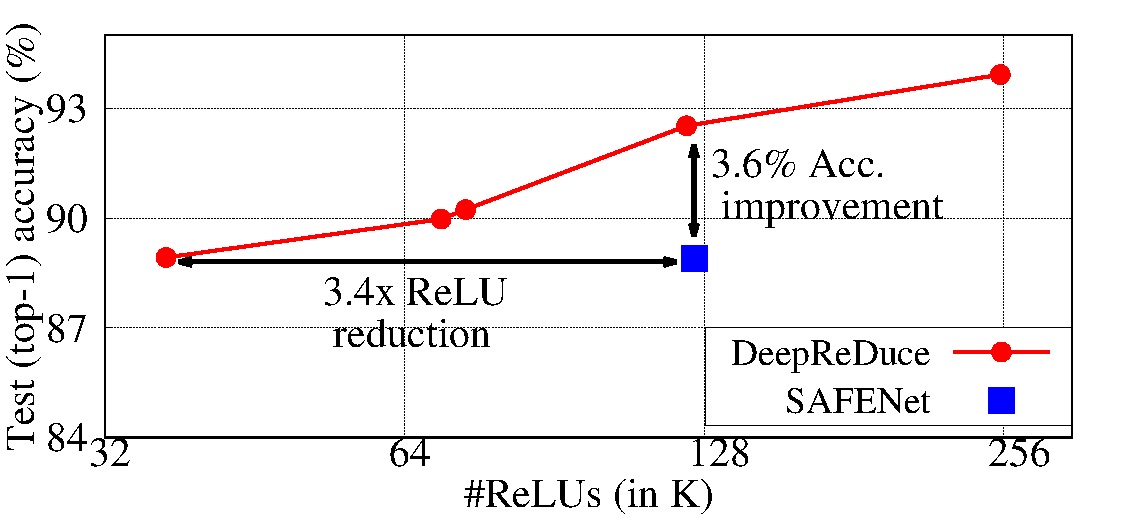
\includegraphics[scale=0.45]{Figures/ParetoFrontier_vgg16}
\vspace{-2em}
\caption{
Performance comparison of VGG16 DeepReDuce model and SAFENet on CIFAR-10. The DeepReDuce-optimized VGG16 models outperform SAFENet-optimized VGG16 by a huge margin at both iso-accuracy and iso-ReLU.}
\vspace{-2em}
\label{fig:ParetoFrontierVGG16}
\end{figure}

%
%
%\textcolor{red}{
%Comparing the online latency for ResNet,  DeepReDuce is {\em 12.86$\times$ faster} (0.56s vs 7.2s) and {\em 1.18\% more accurate} (68.68\% vs 67.5\%). For VGG16,  SAFENet reports 88.9\% accuracy with 56\% ReLUs approximated; even assuming all SAFENet approximated ReLUs are free, DeepReDuce provides a 3.4$\times$ ReLU reduction at iso-accuracy and 3.6\% more accuracy at iso-ReLU count (Figure \ref{fig:ParetoFrontierVGG16}). }

%\begin{figure}[t] \centering
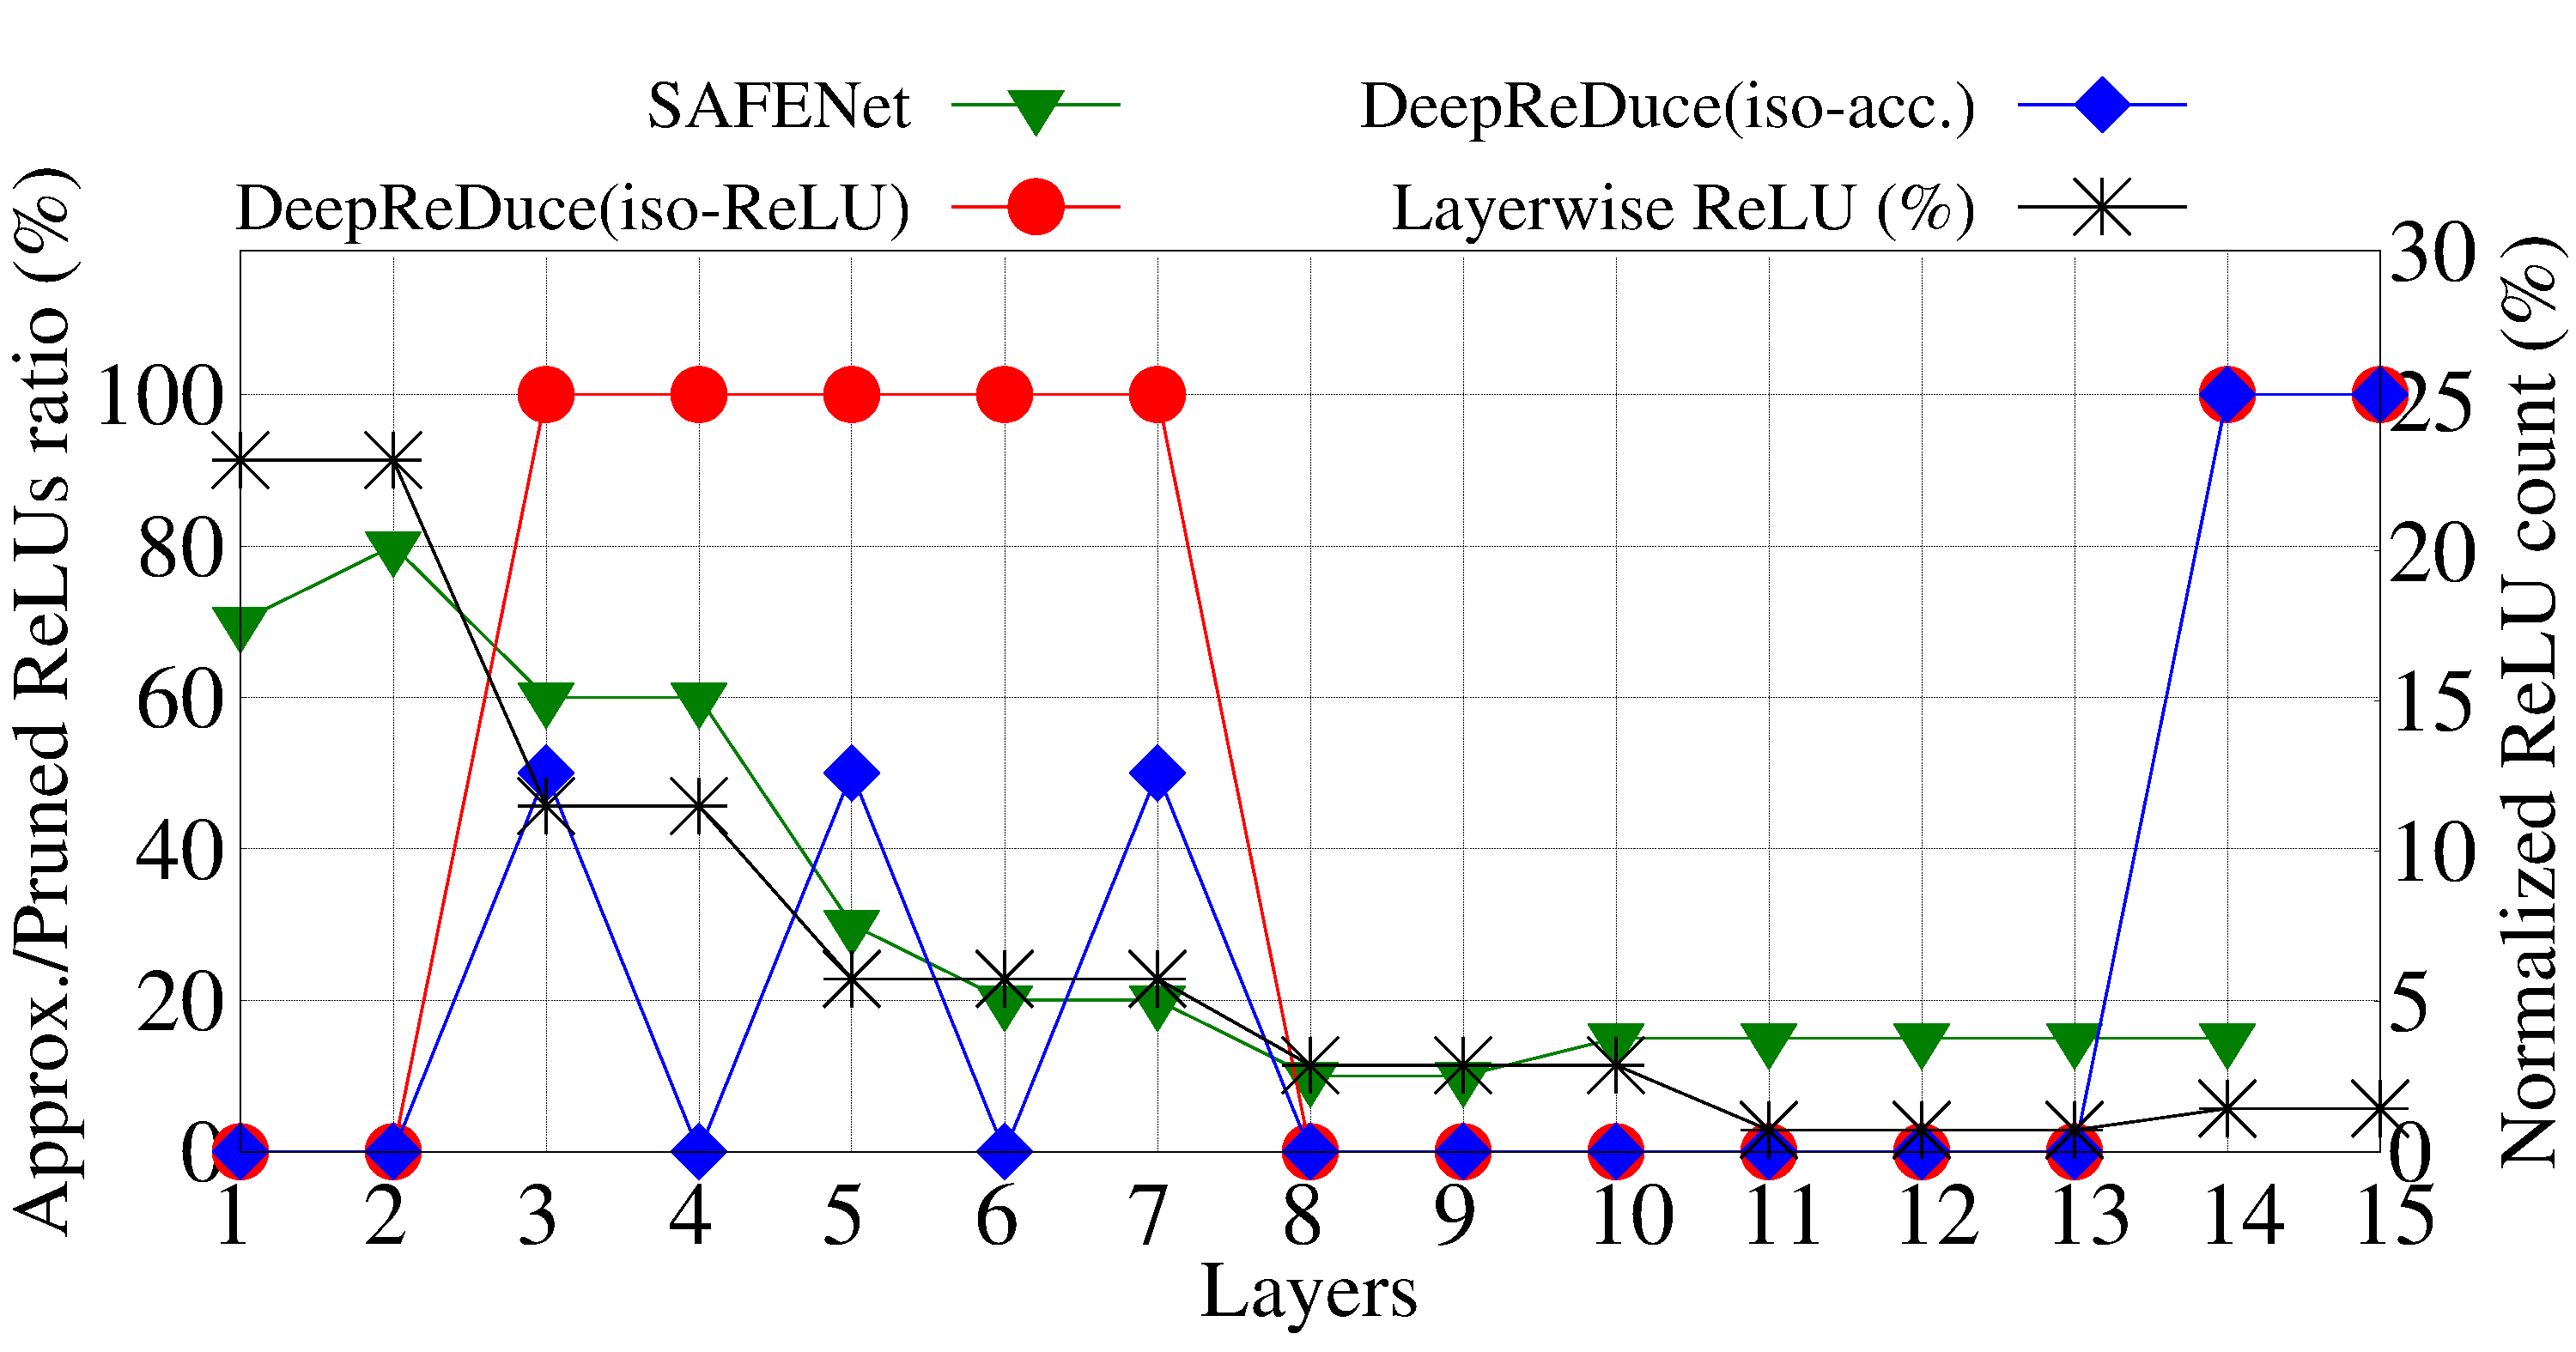
\includegraphics[scale=0.15]{Figures/Safenet_layerwise_comp}
\vspace{-1em}
\caption{Layer-wise approximation/pruned-ReLUs in SAFENet and DeepReDuce models (iso-ReLU and iso-accuracy).  
}
\vspace{-1em}
\label{fig:SafenetLayerwiseComp}
\end{figure}

%\textcolor{red}{
%To understand the effectiveness of DeepReDuce, we compare the layer-wise ReLU distribution in SAFENet and DeepReDuce in Figure \ref{fig:SafenetLayerwiseComp}. Based on the criticality evaluation (Table \ref{tab:ReluCriticalityVGG16} in Appendix \ref{SecAppendix:ParetoPointsVGG16}), we drops all the ReLUs in less critical stages ($S_1$, $S_4$, and $S_5$) and retain the ReLUs in more critical stages ($S_2$ and $S_3$). The optimization steps for the pareto points in Figure 
%\ref{fig:ParetoFrontierVGG16} are illustrated in Table \ref{tab:ParetoPointsVGG16} of Appendix \ref{SecAppendix:ParetoPointsVGG16}. Thus, DeepReDuce models prune all the ReLUs in first two layers where most of network's ReLU reside; however, SAFENet model does not able to approximate all the ReLUs with polynomials in first two layers.  }


\subsection{DeepReDuce Network Inference Latencies}

We conclude by showing the inference speedup time improvements offered by DeepReDuce.
Experiments were run to measure the latency for DeepReDuce optimized models using the same experimental setup and private inference protocol as DELPHI ~\cite{mishra2020delphi}.
Table~\ref{tab:ParetoPoints} and Table~\ref{tab:R18OnTinyImageNet} present latency results of ResNet18 on CIFAR-100 and TinyImageNet, respectively.  
As expected, we observe that inference latency strongly correlates with a network's ReLU count. 
For example, at iso-accuracy (on CIFAR-100), we achieve a 3.7$\times$ latency reduction compared to CryptoNAS. 
Compared to DELPHI, and assuming iso-latency, DeepReDuce offers 3.5\% accuracy improvement on CIFAR-100. 
The fastest DeepReDuce model on CIFAR-100, i.e., the one with the fewest ReLUs, takes 455mS per inference with an accuracy of 65\%.  
Similarly, on TinyImageNet, we achieve 59.18\% top-1 accuracy with a latency of 4.6S.
While advancing the state-of-the-art, these inference times are still too high to meet real-time requirements 30-60 FPS~\cite{edgeFB}, and more work is needed to achieve the ultimate goal of real-time private inference.


\subsection{Generality Case Study: MobileNets}
Here we examine the generality of DeepReDuce using MobileNetV1 \cite{howard2017mobilenets}.
We chose to study MobileNet as it is very different from ResNet---the convolution layers
do not use residuals and the Depthwise architecture is FLOP optimized, which we believe is a poor match for the ReLU costs of private inference.
%types (a non-residual network with FLOPs-optimized Depthwise separable convolution) are significantly different than that of ResNet models.
We first evaluate the ReLUs' criticality (see Table \ref{tab:CriticalityInMobileNets} in Appendix \ref{SecAppendix:ParetoPointsMV1}) and then compare the performance of ReLU-optimized DeepReDuce models with conventionally (channel/fmap-resolution) scaled MobileNetV1 models. For fair comparison, we use KD for scaled-MobileNetV1 models where teacher is Full-ReLU baseline MobileNetV1 and hence, all the results reported in Figure\ref{fig:ParetoFrontierMV1} are with KD.  


Results are shown in Figure \ref{fig:ParetoFrontierMV1} and the optimization steps for all DeepReDuce models are listed in Table \ref{tab:ParetoPointsMV1} in Appendix \ref{SecAppendix:ParetoPointsMV1}. 
The substantial gain, 10.9\% improvement in accuracy at iso-ReLU and 3.8$\times$ ReLU reduction at iso-accuracy (see Figure \ref{fig:ParetoFrontierMV1}) shows the effectiveness of DeepReDuce ReLU optimization on MobileNetV1. 


Thus, while residual connections benefit DeepReDuce, they are not
a necessity as DeepReDuce also performs well when residual connections are eliminated from the network and the non-residual networks such as MobileNets and VGG16 (Figure \ref{fig:ParetoFrontierVGG16}).

% \subsection{ResNet with KD Outperforms State-of-the-art in Private Inference}

% We selected ResNet (as baseline) for our experimentation because of its efficacy in various computer-vision tasks, which is also corroborated by the results shown in  Figure \ref{fig:ParetoFrontierWithKD}. The (scaled) ResNets trained with KD, under the supervision of full ReLU ResNet18 as a teacher, surpass the accuracy of CryptoNAS and DELPHI at iso-ReLU counts. This suggest that with appropriate depth, width, and fmaps' resolution scaling in conjunction with the KD, the classical ResNets can outperform the sophisticated NAS-based ReLU-optimization methods such as CryptoNAS and DELPHI. 

% However, as illustrated in Figure \ref{fig:ParetoFrontierWithKD}, with lower ReLU counts the accuracy gain through KD in ResNets start diminishing. In contrast,  DeepReDuce models maintain the ReLU-accuracy trade-off even at very low ReLU counts and their performance does not degrade sharply.  



%\input{19Figure_ParetoFrontierWithKD}





